
\documentclass[12pt]{article}
\usepackage[a4paper, margin=.30in]{geometry}
\usepackage{graphicx ,
            wrapfig,
            xcolor, 
            enumerate,
            amsmath,
			fontenc,
			tcolorbox,circuitikz
            }
            \usepackage{pgfplots}
\pgfplotsset{compat=1.17}

\newcommand\headerMe[2]{\noindent{}#1\hfill#2}
\renewcommand{\thesection}{\Roman{section}}

\author{Zakaria HAOUZAN}
\date{\today}

\begin{document}
% headers --------------
\headerMe{Matière : Physique-Chimie}{Professeur : Zakaria HAOUZAN}\\
\headerMe{Unité : Electricité }{Établissement : Lycée SKHOR qualifiant}\\
\headerMe{Niveau : 2BAC-SM-PC}{Heure : 7H}\\

% ------Content ________
\begin{center}

    \Large{Leçon $N^{\circ} 4 $: \color{red} Oscillations Forcées dans un Circuit RLC Série }
\end{center}


\section{Le Régime Alternatif Sinusoïdal}

\subsection{La Tension Alternative Sinusoïdale}
La tension alternative sinusoïdale est une fonction du temps qui s'écrit sous la forme suivante :
\begin{equation}
    u(t) = U_m\cos(\omega t + \phi_u)
\end{equation}



\begin{center}
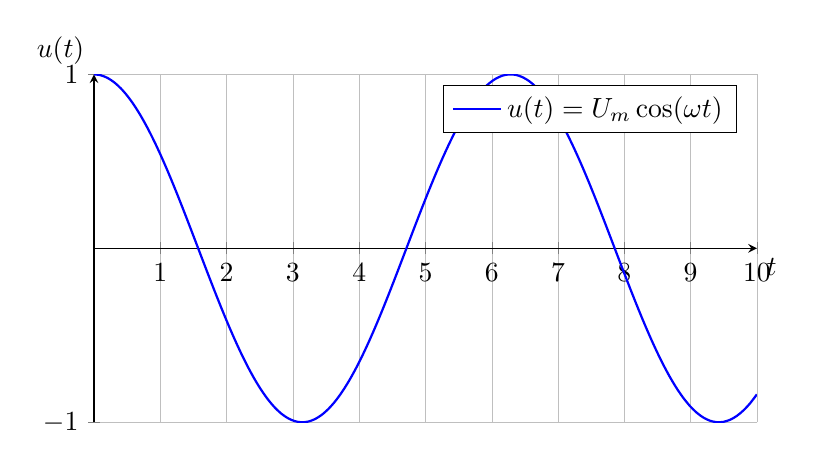
\begin{tikzpicture}
    \begin{axis}[
        axis lines=middle,
        xlabel={$t$},
        ylabel={$u(t)$},
        xlabel style={below right},
        ylabel style={above left},
        xtick={0, 1, 2, 3, 4, 5, 6, 7, 8, 9, 10},
        ytick={-1, 0, 1},
        domain=0:10,
        samples=100,
        width=10cm,
        height=6cm,
        grid=both,
        major grid style={line width=.2pt,draw=gray!50},
        minor grid style={line width=.1pt,draw=gray!25},
        legend pos=north east,
    ]
    \addplot[
        blue,
        thick,
        smooth
    ]{cos(deg(x))}; % Zero phase shift
    \addlegendentry{$u(t) = U_m \cos(\omega t)$}
    \end{axis}
\end{tikzpicture}
\end{center}

\section*{I) Le régime alternatif sinusoïdal}

\subsection*{1) La tension alternative sinusoïdale}
La tension alternative sinusoïdale est une fonction du temps, qui s'écrit sous la forme suivante :
\[ u(t) = U_m\cos(\omega t + \phi_u) \]

$U_m$ : L'amplitude de u(t) en volts (V) ;\\
$\omega$ : La pulsation de u(t) en (rad.s$^{-1}$) avec $\omega = \frac{2\pi}{T} = 2\pi f$ ;\\
$(\omega t + \phi_u)$ : La phase de u(t) à l'instant t en (rad) ;\\
$\phi_u$ : La phase de la tension à l'origine des temps en (t=0).

La tension efficace U d'une tension alternative sinusoïdale est donnée par la relation suivante : 
\[ U = \frac{U_m}{\sqrt{2}} \]

\textbf{Remarque} : Le voltmètre indique la valeur efficace de la tension et l'oscilloscope indique la tension maximale.

\subsection*{2) Intensité du courant alternatif sinusoïdal}
L'intensité du courant alternatif sinusoïdal est une fonction du temps qui s'écrit sous la forme suivante :
\[ i(t) = I_m\cos(\omega t + \phi_i) \]

$I_m$ : L'amplitude ou l'intensité maximale du courant en ampère (A) ;\\
$\omega$ : La pulsation du courant en (rad.s$^{-1}$) avec $\omega = \frac{2\pi}{T} = 2\pi f$ ;\\
$(\omega t + \phi_i)$ : La phase de i(t) à l'instant t en (rad) ;\\
$\phi_i$ : La phase de l'intensité à l'origine des temps (t=0).

L'intensité efficace I d'un courant alternatif sinusoïdal est donnée par la relation suivante : 
\[ I = \frac{I_m}{\sqrt{2}} \]

\textbf{Remarque} : L'ampèremètre indique la valeur efficace d'intensité.

\subsection*{3) Notion de la phase}
On considère deux grandeurs alternatives sinusoïdales :
\[ u(t) = U_m\cos(\omega t + \phi_u) \text{ et } i(t) = I_m\cos(\omega t + \phi_i) \]

On appelle la phase de la tension u(t) par rapport à l'intensité i(t) : $\phi_{u/i} = \phi_u - \phi_i$ (mesure l'avance et le retard de la tension u(t) par rapport à l'intensité i(t))

Pour simplifier l'étude, on prend $\phi_i = 0$ alors $\phi_{u/i} = \phi_u$
\[ u(t) = U_m\cos(\omega t + \phi_u) \Leftrightarrow u(t) = U_m\cos(\omega(t + \frac{\phi_u}{\omega})) \]

On appelle $\frac{\phi_u}{\omega}$ le retard $\tau = \frac{\phi_u}{\omega}$ avec $\omega = \frac{2\pi}{T}$ donc $\phi_{u/i} = \phi_u = \tau\frac{2\pi}{T}$

Pratiquement la mesure de $\tau$ par l'oscilloscope nous permet de déterminer la valeur absolue de $\phi_{u/i}$.

  \begin{center}
    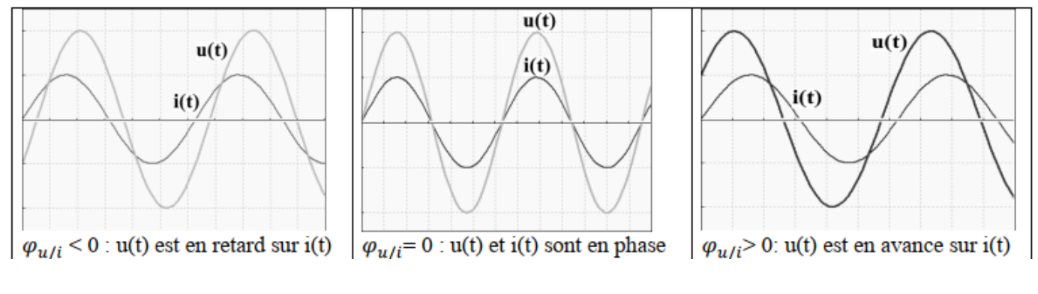
\includegraphics[width=0.9\textwidth]{./img/phase partie.png}
  \end{center}


\section*{II) Etude expérimentale du circuit RLC série en régime alternatif sinusoïdal}

\subsection*{1) Oscillations forcées dans un circuit RLC}
On alimente le circuit RLC série avec un générateur basse fréquence (GBF) délivrant une tension sinusoïdale $u(t) = U_m\cos(\omega t + \phi_u)$ et on visualise les tensions $u_R(t)$ sur la voie Y$_1$ et u(t) sur la voie Y$_2$ d'un oscilloscope.

  \begin{center}
    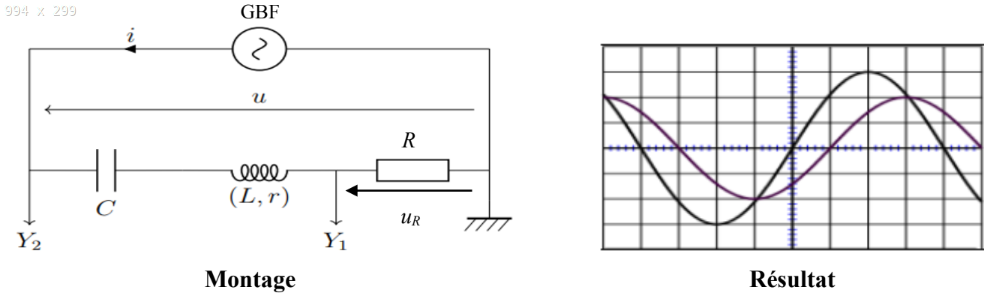
\includegraphics[width=0.9\textwidth]{./img/montage.png}
  \end{center}



En faisant varier la fréquence du GBF, on remarque, en utilisant les oscillogrammes, que les deux tensions u(t) et $u_R(t)$ ont la même période (même fréquence), on dit que les oscillations de la tension $u_R(t)$ sont imposées par le générateur, l'oscillateur n'est pas libre et les oscillations sont dites forcées.

\textbf{Conclusion}
\begin{itemize}
\item La fréquence des oscillations est imposée par le générateur : on dit que les oscillations sont forcées.
\item Le générateur joue le rôle de l'excitateur.
\item Le dipôle RLC en série joue le rôle du résonateur.
\item L'excitateur fournit de l'énergie au résonateur pour compenser l'énergie perdue par effet Joule.
\end{itemize}

\subsection*{2) Notion d'impédance}
L'impédance d'un dipôle est égale au quotient de la valeur efficace de la tension à ses bornes par la valeur efficace de l'intensité : 
\[ Z = \frac{U}{I} = \frac{U_m}{I_m} \]

L'impédance dépend de la fréquence du circuit.

L'unité de l'impédance dans le système internationale est $\Omega$.

\textbf{Remarque} : Théoriquement l'expression de l'impédance d'un circuit RLC à la fréquence f est :
\[ Z = \sqrt{R^2 + (L2\pi f - \frac{1}{C2\pi f})^2} \]

\section*{III) Phénomène de résonance d'intensité}

\subsection*{1) Phénomène de résonance}
Lorsque la fréquence f d'excitateur prend une valeur égale à la fréquence propre $f_0$ du résonateur, l'intensité efficace I du courant qui traverse le circuit sera maximale et égale à $I_0$, on dit dans ce cas que le circuit RLC série est en résonance.

Donc : $f = f_0 = \frac{1}{2\pi\sqrt{LC}}$

\subsection*{2) L'impédance du circuit RLC à la résonance}
\begin{itemize}
\item À la résonance, l'intensité efficace I du courant qui traverse le circuit sera maximale alors l'impédance passe par la valeur minimale.
\item À la résonance, l'impédance du circuit RLC est égale à la résistance globale du circuit : Z = R
\end{itemize}
  \begin{center}
    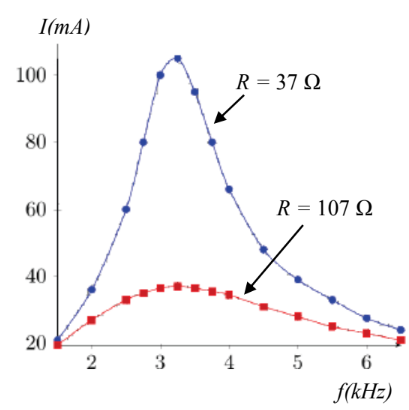
\includegraphics[width=0.38\textwidth]{./img/Resonancefig1.png}
    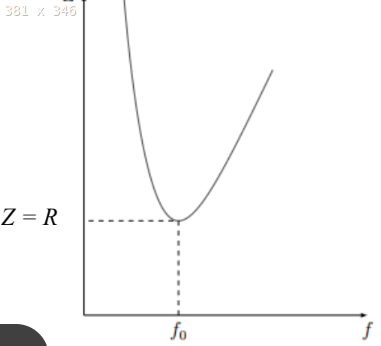
\includegraphics[width=0.38\textwidth]{./img/Reso.png}
  \end{center}


\textbf{Remarque}
\begin{itemize}
\item À la résonance, le circuit RLC se comporte comme un conducteur ohmique de résistance R.
\item À la résonance la tension aux bornes du condensateur est égale à la tension aux bornes de la bobine :
\[ U_L = U_C \text{ donc } L\omega_0 = \frac{1}{C\omega_0} \Leftrightarrow L\cdot2\pi f_0 = \frac{1}{C\cdot2\pi f_0} \]
\end{itemize}


\subsection*{3) La phase à la résonance}
À la résonance l'intensité i(t) et la tension u(t) sont en phase :
$\phi_{u/i} = 0$

\textbf{Remarque} :
D'après la courbe de la résonance d'intensité et l'étude expérimentale si :
\begin{itemize}
\item f $\leq$ $f_0$ on a i(t) en avance de phase sur u(t) on dit que le circuit est capacitif.
\item f $\geq$ $f_0$ on a u(t) en avance de phase sur i(t) on dit que le circuit est inductif.
\end{itemize}

\subsection*{4) La bande passante à -3db du circuit RLC}
\subsubsection*{a) Définition}
La bande passante à -3db du circuit RLC est définie comme une intervalle continue des fréquences [$f_1$, $f_2$] du générateur, pour laquelle l'intensité efficace I du courant vérifie la relation suivante : 
\[ I \geq \frac{I_0}{\sqrt{2}} \]
où $I_0$ est l'intensité maximale efficace du courant à la résonance.

\subsubsection*{b) La largeur de bande passante -3db}
  \begin{center}
    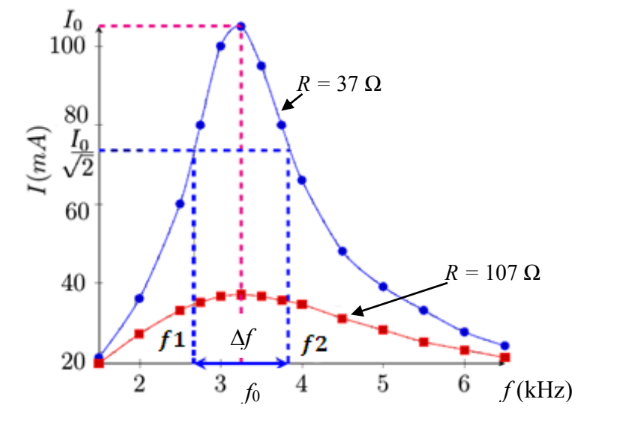
\includegraphics[width=0.68\textwidth]{./img/largeur.png}
  \end{center}




On conclue que :
\begin{itemize}
\item Dans le cas où R est petite (amortissement faible), la résonance est aiguë et la largeur de la bande passante $\Delta f$ est petite.
\item Dans le cas où R est grande (amortissement forte), la résonance est floue et $\Delta f$ est grande.
\end{itemize}

\textbf{Remarque}
Théoriquement l'expression de la bande passante -3db est donnée par la relation :
\[ \Delta\omega = \omega_2 - \omega_1 = \frac{R}{L} \]
\[ \Delta f = \frac{\Delta\omega}{2\pi} = \frac{R}{2\pi L} \]

\subsection*{5) Facteur de qualité}
On définit le facteur de qualité Q par un nombre sans dimension : 
\[ Q = \frac{\omega_0}{\Delta\omega} \text{ ou } Q = \frac{f_0}{\Delta f} \]

Avec $\omega_0$ et $f_0$ sont respectivement la pulsation propre et la fréquence propre. $\Delta\omega$ ou $\Delta f$ la largeur de la bande passante.

\begin{itemize}
\item Puisque $\Delta\omega = \frac{R}{L}$ alors le facteur de qualité Q sera : 
\[ Q = \frac{L\omega_0}{R} = \frac{L\cdot2\pi f_0}{R} \]
\item À la résonance : $L\cdot2\pi f_0 = \frac{1}{C\cdot2\pi f_0}$ alors le facteur de qualité Q sera : 
\[ Q = \frac{1}{R\cdot C\cdot2\pi f_0} = \frac{1}{R\cdot C\cdot\omega_0} \]
\item La fréquence propre $f_0 = \frac{1}{2\pi\sqrt{LC}}$ alors le facteur de qualité Q sera : 
\[ Q = \frac{1}{R}\sqrt{\frac{L}{C}} \]
\end{itemize}

\textbf{Remarque}
À la résonance, le circuit RLC se comporte comme un conducteur ohmique de résistance R, donc la tension efficace : U = R$I_0$
\[ Q = \frac{L\omega_0}{R}\frac{I_0}{I_0} = \frac{1}{R\cdot C\cdot\omega_0}\frac{I_0}{I_0} = \frac{U_L}{U} = \frac{U_C}{U} \]

On appelle le facteur de qualité : le facteur de surtension car : $U_L = Q\cdot U$

\textbf{Quelques effets de la résonance sur le circuit}\\
Le facteur de qualité Q est inversement proportionnel à la largeur de la bande passante et qui caractérise l'acuité de la résonance.
\begin{itemize}
\item Si Q est grand alors le circuit est plus sélectif.
\item Si la résonance est aiguë alors la valeur de Q est grande.
\item Si la résonance est floue alors le circuit est amorti.
\end{itemize}



\section*{IV) La puissance en régime alternatif sinusoïdal}

\subsection*{1) La puissance instantanée}
On considère un dipôle AB traversant un courant alternatif sinusoïdal : $i(t) = I\sqrt{2}\cos(\omega t)$ et la tension à ses bornes $u(t) = U\sqrt{2}\cos(\omega t + \phi)$.

En convention récepteur, la puissance instantanée reçue par un dipôle s'écrit : P(t) = u(t)$\cdot$i(t)

P(t) = u(t)$\cdot$i(t) = 2UI$\cdot$cos($\omega$t + $\phi$)$\cdot$cos($\omega$t)

Puisque : cos a$\cdot$cos b = $\frac{1}{2}$[cos(a + b) + cos(a - b)]

Alors P(t) = U$\cdot$I[cos $\phi$ + cos(2$\omega$t + $\phi$)]

La puissance est une fonction sinusoïdale de pulsation 2$\omega$ et de période $\frac{T}{2}$ avec T la période de u(t) et i(t).

\subsection*{2) La puissance moyenne ou puissance active}
La puissance moyenne est la somme des puissances instantanées consommées par un dipôle durant la période T.
\[ P = \frac{1}{T}\int_0^T P(t)dt = \frac{1}{T}\int_0^T UI[\cos\phi + \cos(2\omega t + \phi)]dt \]
\[ = \frac{UI}{T}(\cos\phi\cdot T + [\frac{1}{2\omega}\sin(2\omega t + \phi)]_0^T) \]
\[ = UI\cos\phi + \frac{UI}{T}\cdot\frac{1}{2\omega}(\sin(2\omega T + \phi) - \sin\phi) \]

Puisque sin(2$\omega$T + $\phi$) = sin(4$\pi$ + $\phi$) = sin $\phi$

Alors la puissance moyenne a pour expression : P = U$\cdot$I$\cdot$cos $\phi$

  \begin{itemize}
\item Le produit U$\cdot$I des amplitudes efficaces désigne la puissance apparente S du dipôle : S = U$\cdot$I
\item Le cos $\phi$ correspond au facteur de puissance.
\end{itemize}

Puisque U = Z$\cdot$I et cos $\phi$ = $\frac{R}{Z}$ donc on a : P = Z$\cdot$I$\cdot$I$\cdot\frac{R}{Z}$ = R$\cdot$I$^2$

Dans un circuit RLC série la puissance électrique moyenne ne se consomme que par la résistance globale R par effet joule et elle est donnée par la relation suivante : P = R$\cdot$I$^2$


\end{document}

